% ---------------------------------------------------------------------------- %
\chapter{Test Bench}
\label{chap:testBench}
% ---------------------------------------------------------------------------- %

This chapter presents a brief overview of  the test bench and provides a guide
on how to put it into operation.

A detailled list  of all the devices, components and  software which were used
to obtain  the measurements  from Chapter  \ref{chap:results} is  given, along
with information on how to make all those pieces work.  This chapter therefore
answers  the  questions  \emph{What did  we  use,  and  how  does it  all  fit
together?}, whereas  the measurement  methodology (\emph{What  did we  do with
it?}) will be answered in the next chapter.

Fundamentally,   there   are   two    kinds   of   measurements: Digital   and
analog. The  digital  measurements consist  of  the  bit stream,  whereas  the
analog  measurements   are  concerned   with  measuring   the  pre-amplifier's
characteristics. For the most  part, the test benches for  these two scenarios
are identical.  The  primary difference is that for  the digital measurements,
the bit  stream is  measured on  the GPIO pins  of the  \raspi, while  for the
analog measurements, data  is obtained from oscilloscope. This can  be done in
multiple  ways; the  test bench  as implemented  in this  project is  based on
remote-controlling the oscilloscope from a computer.

Unless otherwise  noted, the information  presented in the  following sections
applies to both types of measurements.

% ---------------------------------------------------------------------------- %
\section{Overview}
\label{sec:overview}
% ---------------------------------------------------------------------------- %

The  complete   experimental  setup  as   used  during  our   measurements  is
shown   in  figure   \ref{fig:testBenchComplete}. A  schematic   depiction  of
the   various   connections  between   the   devices   is  shown   in   figure
\ref{fig:testBenchConnections}. The   following  sections   describe  how   to
configure each  of the  components.  Table \ref{tab:componentList}  contains a
list of the devices components which are used.

\begin{figure}
    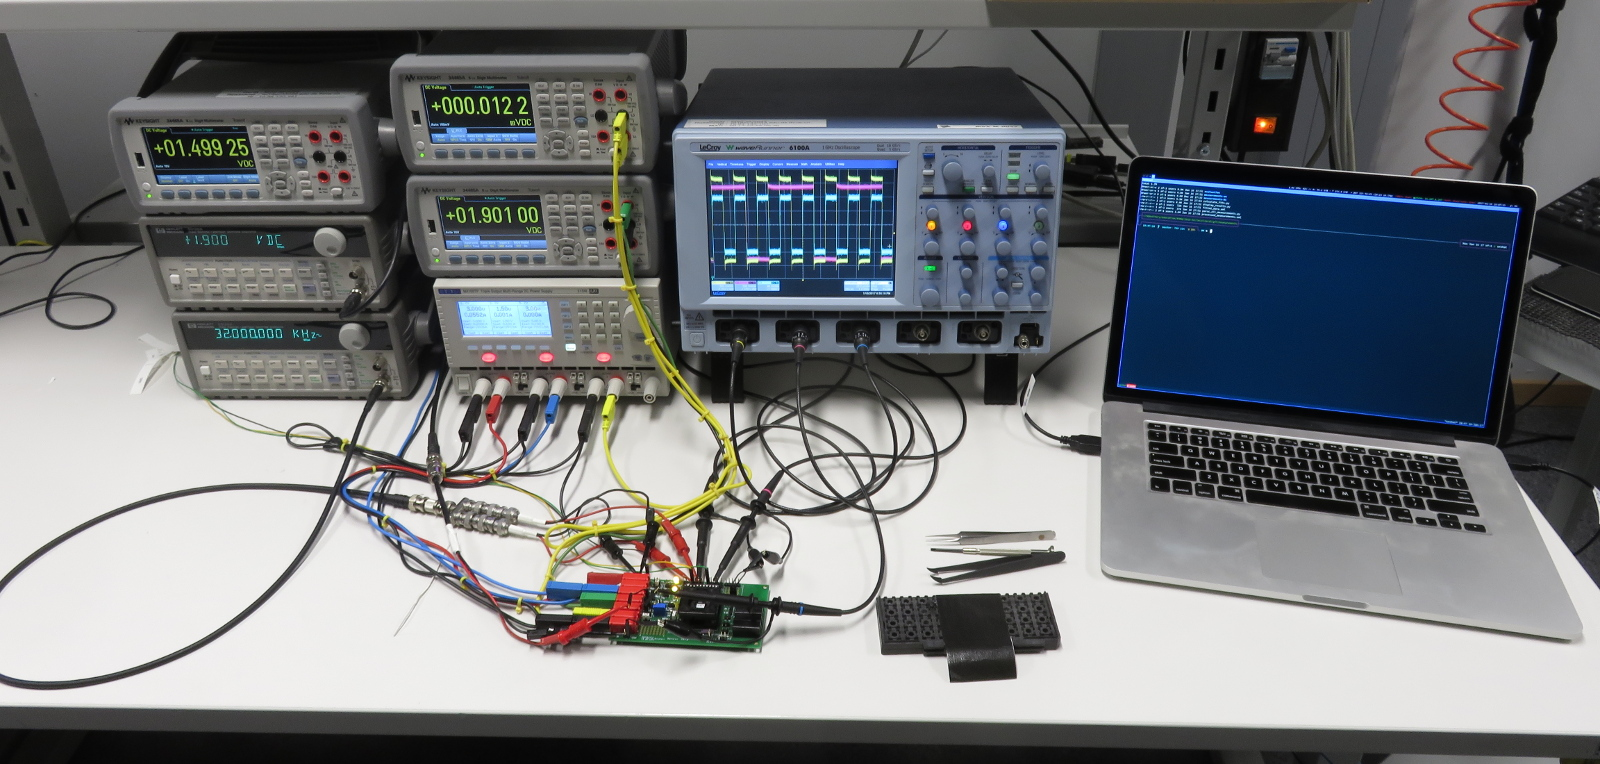
\includegraphics[width=0.9\textwidth]{images/expSetup/testBenchComplete.jpeg}
    \caption{
        The test bench as used in  our measurements. The \raspi~ is behind the
        waveform generators on the left-hand side.%
    }
    \label{fig:testBenchComplete}
\end{figure}

\begin{figure}
    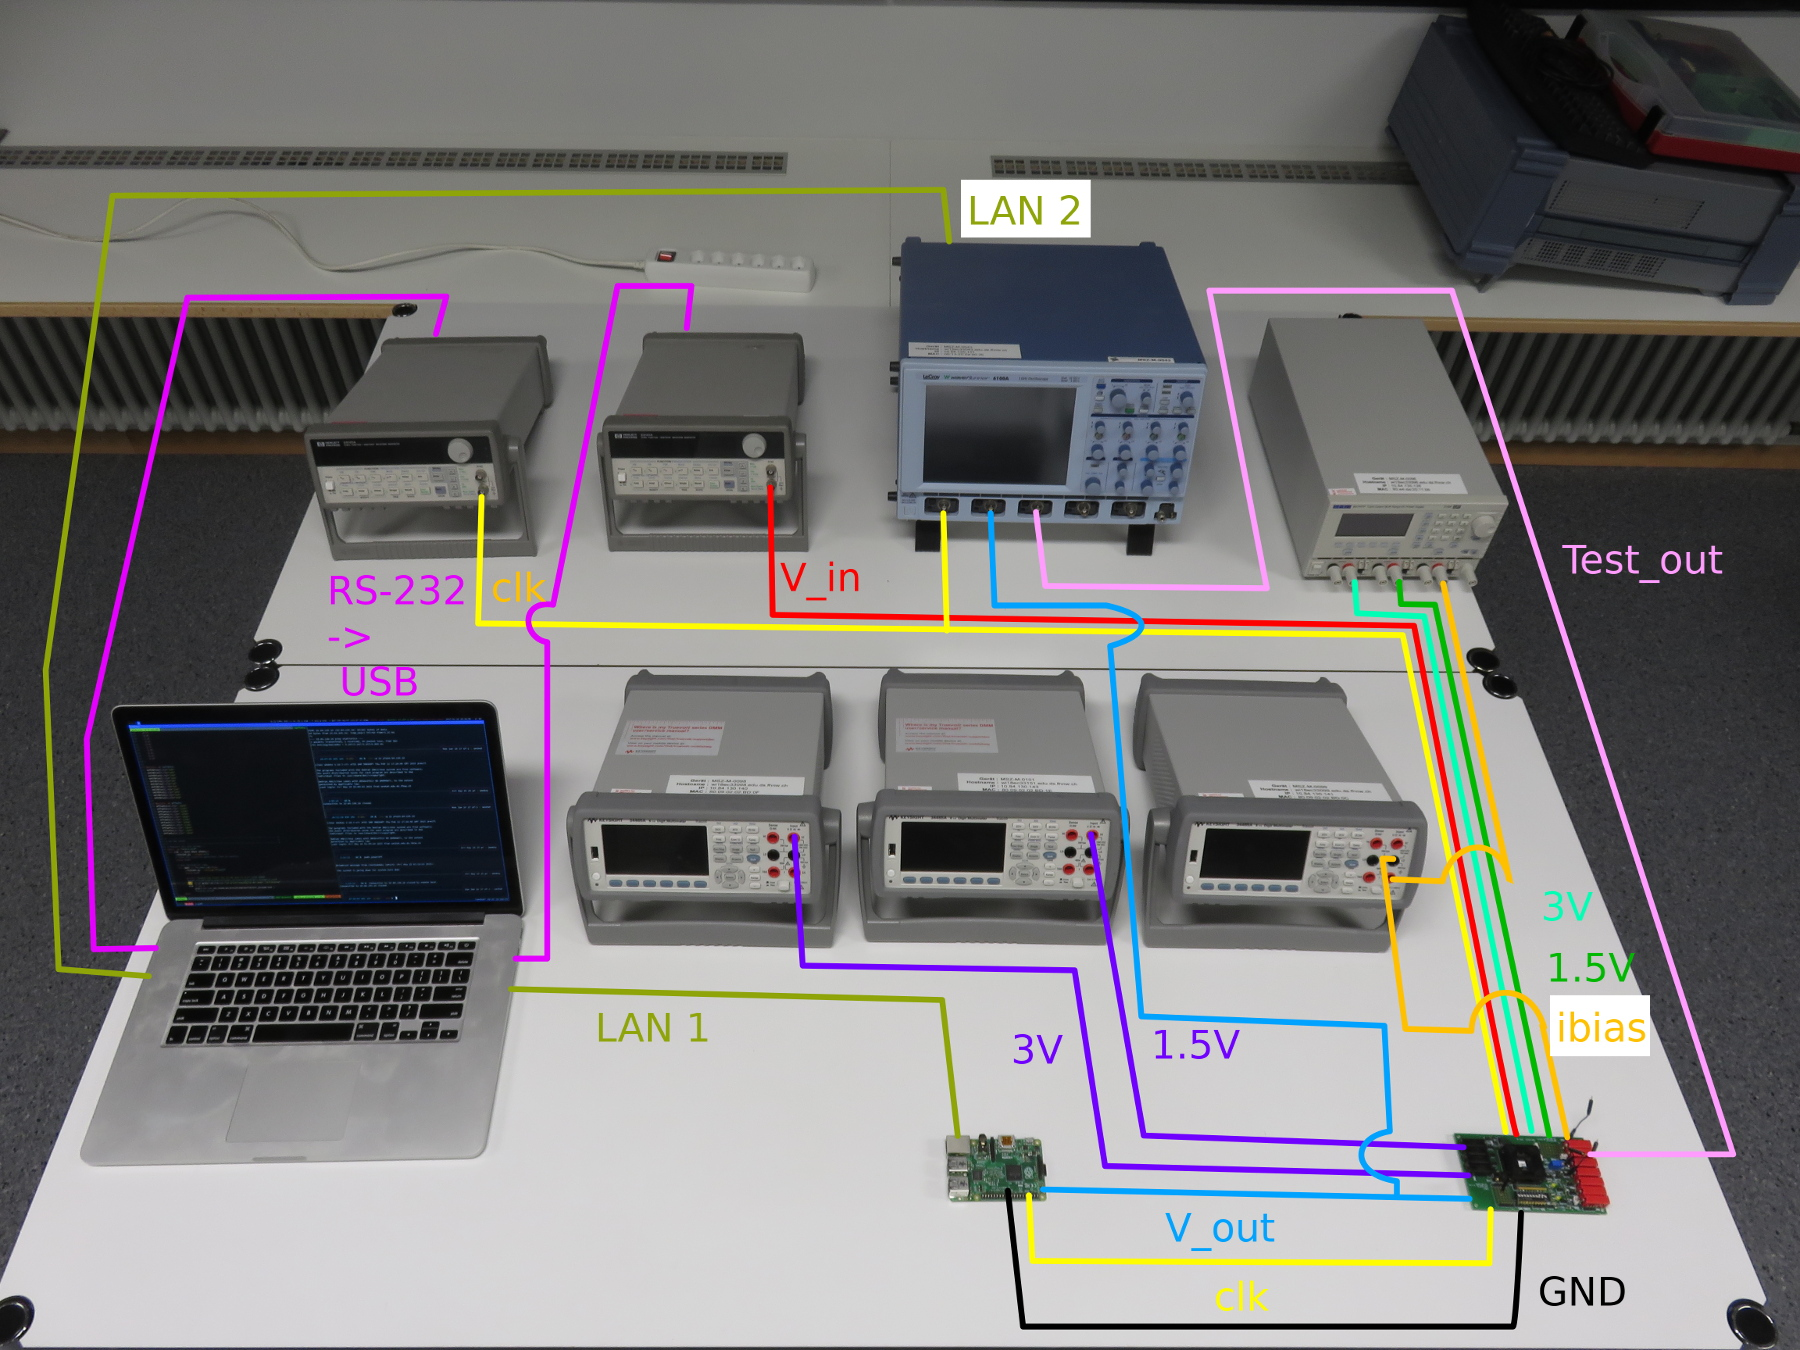
\includegraphics[width=0.9\textwidth]{images/expSetup/testBenchConnections.jpeg}
    \caption{%
        Schematic  connections between  the devices  in the  setup as  used in
        figure  \ref{fig:testBenchComplete}. To  reduce  clutter,  all  ground
        connections except the one between the \raspi~ and the test board have
        been omitted.%
    }
    \label{fig:testBenchConnections}
\end{figure}

\begin{table}
\begin{centering}
    \caption{Component list}
    \label{tab:componentList}
\begin{xtabular}{
    >{\small}p{50mm}
    >{\small}p{8mm}
    >{\small}p{65mm}
}
    \toprule
    \textsc{Item}    &
    \textsc{Count}   &
    \textsc{Notes}   \\
    \midrule

    HP 33120A Arbitrary Waveform Generator  &
    2                                       &
    For generating input signal and clock   \\
 
    Keysight 34465A Tabletop Multimeter                     &
    3                                                       &
    Monitoring \signal{VGNDA}, \signal{VIN}, \signal{IBIAS} \\

    Aim TTi MX100TP DC Power Supply                                         &
    1                                                                       &
    Supply for \signal{VDDD}, \signal{VDDA}, \signal{VGNDA}, \signal{IBIAS} \\

    
    LeCroy waveRunner 6100A 1 GHz Oscilloscope                        &
    1                                                                 &
    Monitoring \signal{CLK}, \signal{TEST\_OUT}, \signal{SIGNAL\_OUT} \\

    Probes for LeCroy waveRunner 6100A                               &
    1                                                                &
    Measuring \signal{CLK}, \signal{TEST\_OUT}, \signal{SIGNAL\_OUT} \\

    Ethernet cable                          &
    1                                       &
    Connecting the oscilloscope to a laptop \\

    Raspberry Pi                                           &
    1                                                      &
    reading and storing bit stream (\signal{SIGNAL\_OUT}), 
    Operating System: Raspbian                             \\

    Laboratory cables with industrial plugs         &
    12                                              &
    Various connections (see diagrams and pictures) \\

    Coaxial Cables (\SI{50}{\ohm})               &
    2                                            &
    Connecting waveform generators to test board \\

    Y-adapter for coaxial cable &
    1                           &
    \\

    Breakout adapters for coaxial cables &
    3                                    &
    \\

    Measuring terminals, small &
    6                          &
    \\

    Test board &
    1          &
    \\

    Sensor IC                       &
    10                              &
    Chips used: C1V1 through C1V10  \\

    USB $\rightarrow$ RS232 adapters                  &
    2                                                 &
    For controlling the waveform generators from a PC \\

    USB cables                                        &
    2                                                 &
    For controlling the waveform generators from a PC,
    USB A $\rightarrow$ USB-B                         \\

    Computer                                                  &
    1                                                         &
    Remote-control for oscilloscope and waveform generators,
    Operating System: Linux  or *BSD with  a bash-compatible
    shell and the necessary Python libraries                  \\

    Hand-held multimeter                         &
    1                                            &
    For monitoring various parameters as needed. \\

    \bottomrule
\end{xtabular}
\end{centering}
\end{table}


% ---------------------------------------------------------------------------- %
\clearpage
\section{Sensor Test Board}
\label{sec:testBoard}
% ---------------------------------------------------------------------------- %

The test board provides a platform for easy operation and configuration of the
sensor chip. It has  inputs for the various supply voltages,  a socket for the
chip itself  and outputs various signals. The  full list of the  chip's pinout
can be found in table \ref{tab:topLevelPins}.

The primary  item to configured  on the test  board are the  DIP switches. The
assignment  key  for them  is  listed  in  table \ref{tab:dipSwitches}  .  The
major  gains  (also  configurable  via  DIP  switches)  are  listed  in  table
\ref{tab:gainSettings}.

The       schematic      for       the      test       board      can       be
found       in       Appendix~\ref{app:testBoardSchematic}       on       page
\pageref{app:testBoardSchematic}.

\begin{table}
    \centering
    \caption{DIP switch assignments}
    \label{tab:dipSwitches}
    \small
    \begin{tabular}{rl}
        \toprule
        Switch No. & Assignment \\
        \midrule
         1 & none \\
         2 & external reset for pre-amplifier \\
         3 & positive/negative sign for pre-amplifier (on: negative)\\
         4 & pre-amplifier bit 3 \\
         5 & pre-amplifier bit 2 \\
         6 & pre-amplifier bit 1 \\
         7 & pre-amplifier bit 0 \\
         8 & sample-and-hold enable \\
         9 & pre-amplifier enable \\
        10 & none \\
        \bottomrule
    \end{tabular}
\end{table}

\begin{table}
    \centering
    \caption{Major gain settings for pre-amplifier}
    \label{tab:gainSettings}
    \small
    \begin{tabular}{p{10mm}p{10mm}p{10mm}p{10mm}p{10mm}}
        \toprule
        $d_3$ & $d_2$ & $d_1$ & $d_0$ & Gain \\
        \midrule
        1 & 1 & 1 & 1 & 1 \\
        0 & 1 & 1 & 1 & 2 \\
        0 & 0 & 1 & 1 & 4 \\
        0 & 0 & 0 & 1 & 8 \\
        0 & 0 & 0 & 0 & 16 \\
        \bottomrule
    \end{tabular}
\end{table}

\begin{figure}
    \centering
    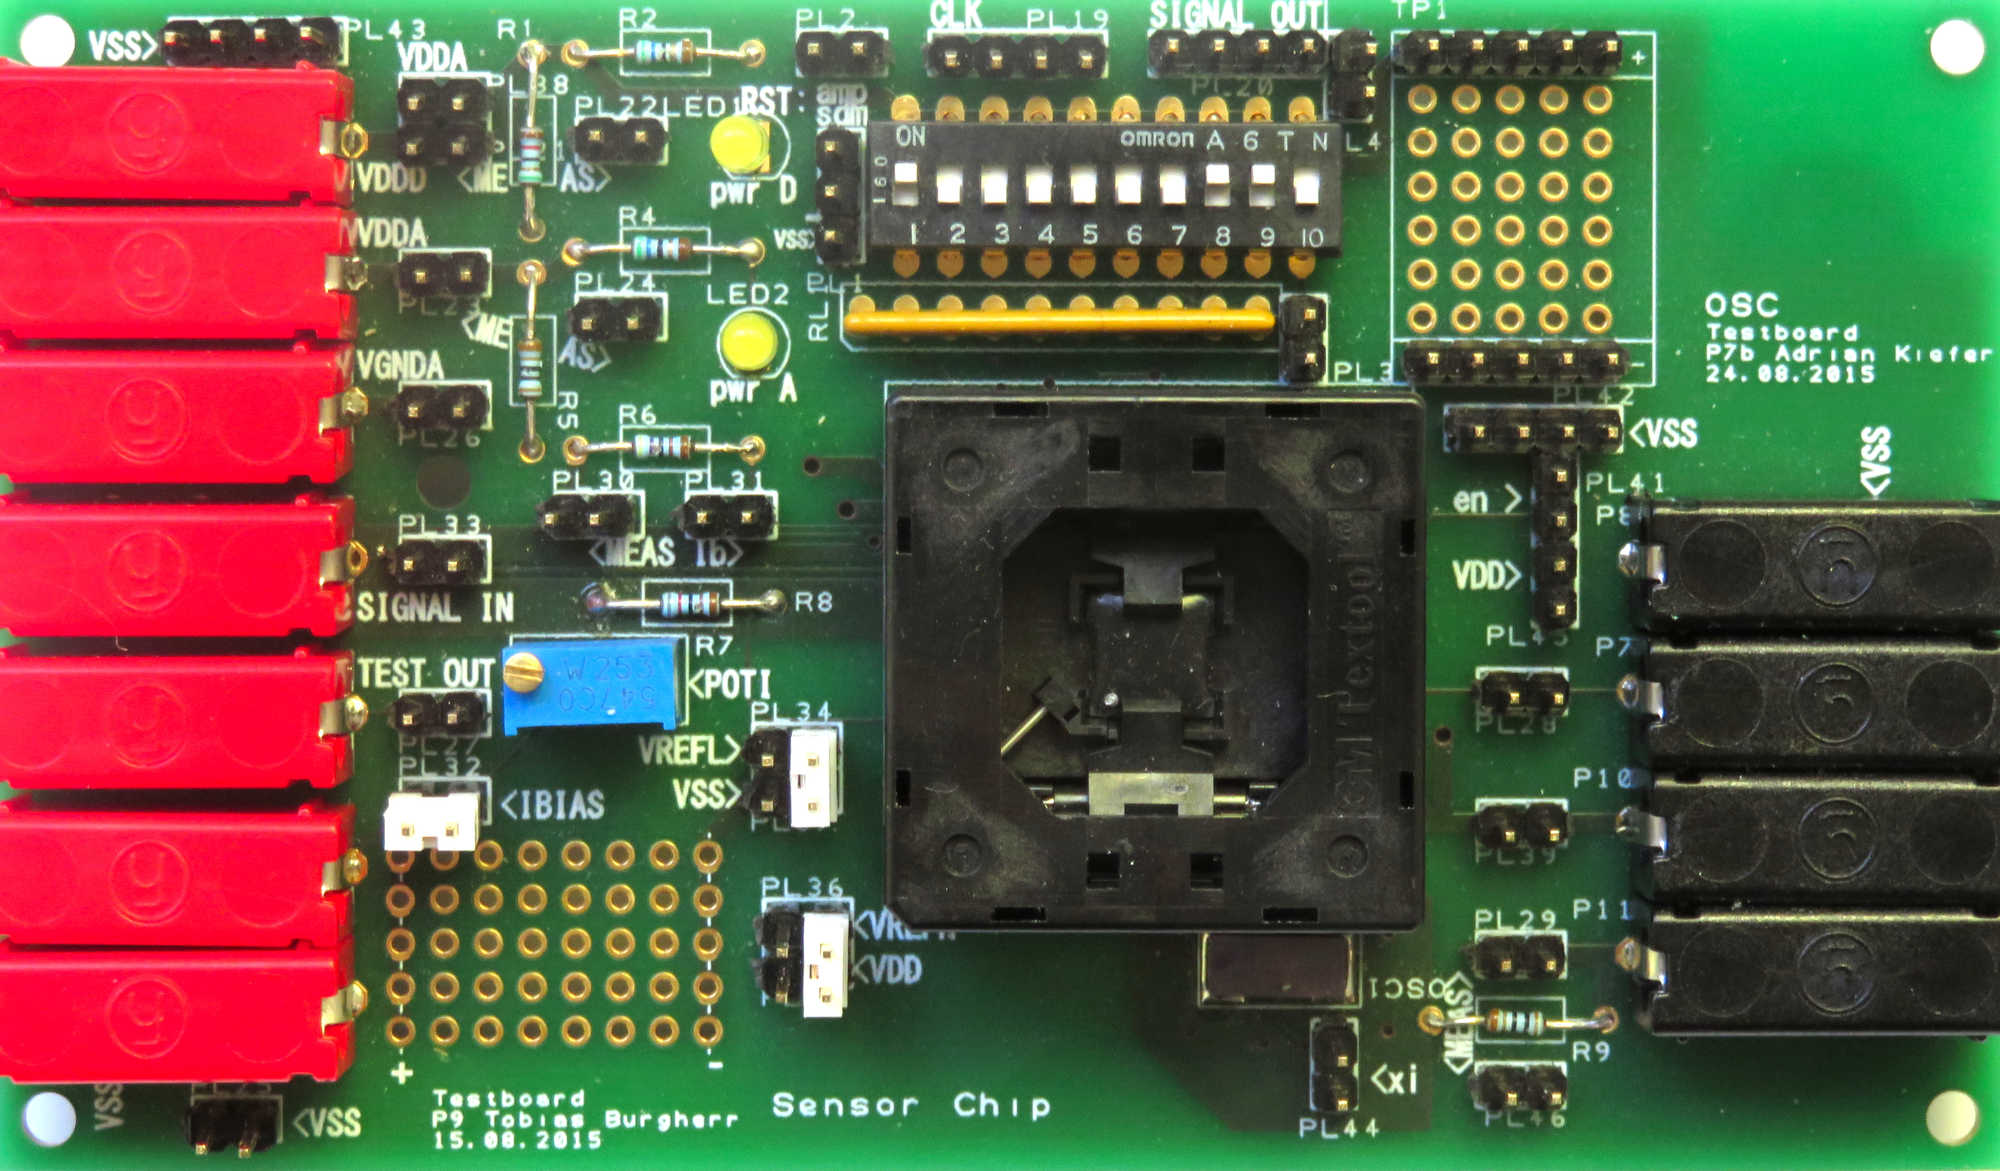
\includegraphics[width=0.9\textwidth]{images/pcb/pcbOverview}
    \caption{The test board.}
    \label{fig:testBoard}
\end{figure}

\begin{figure}
    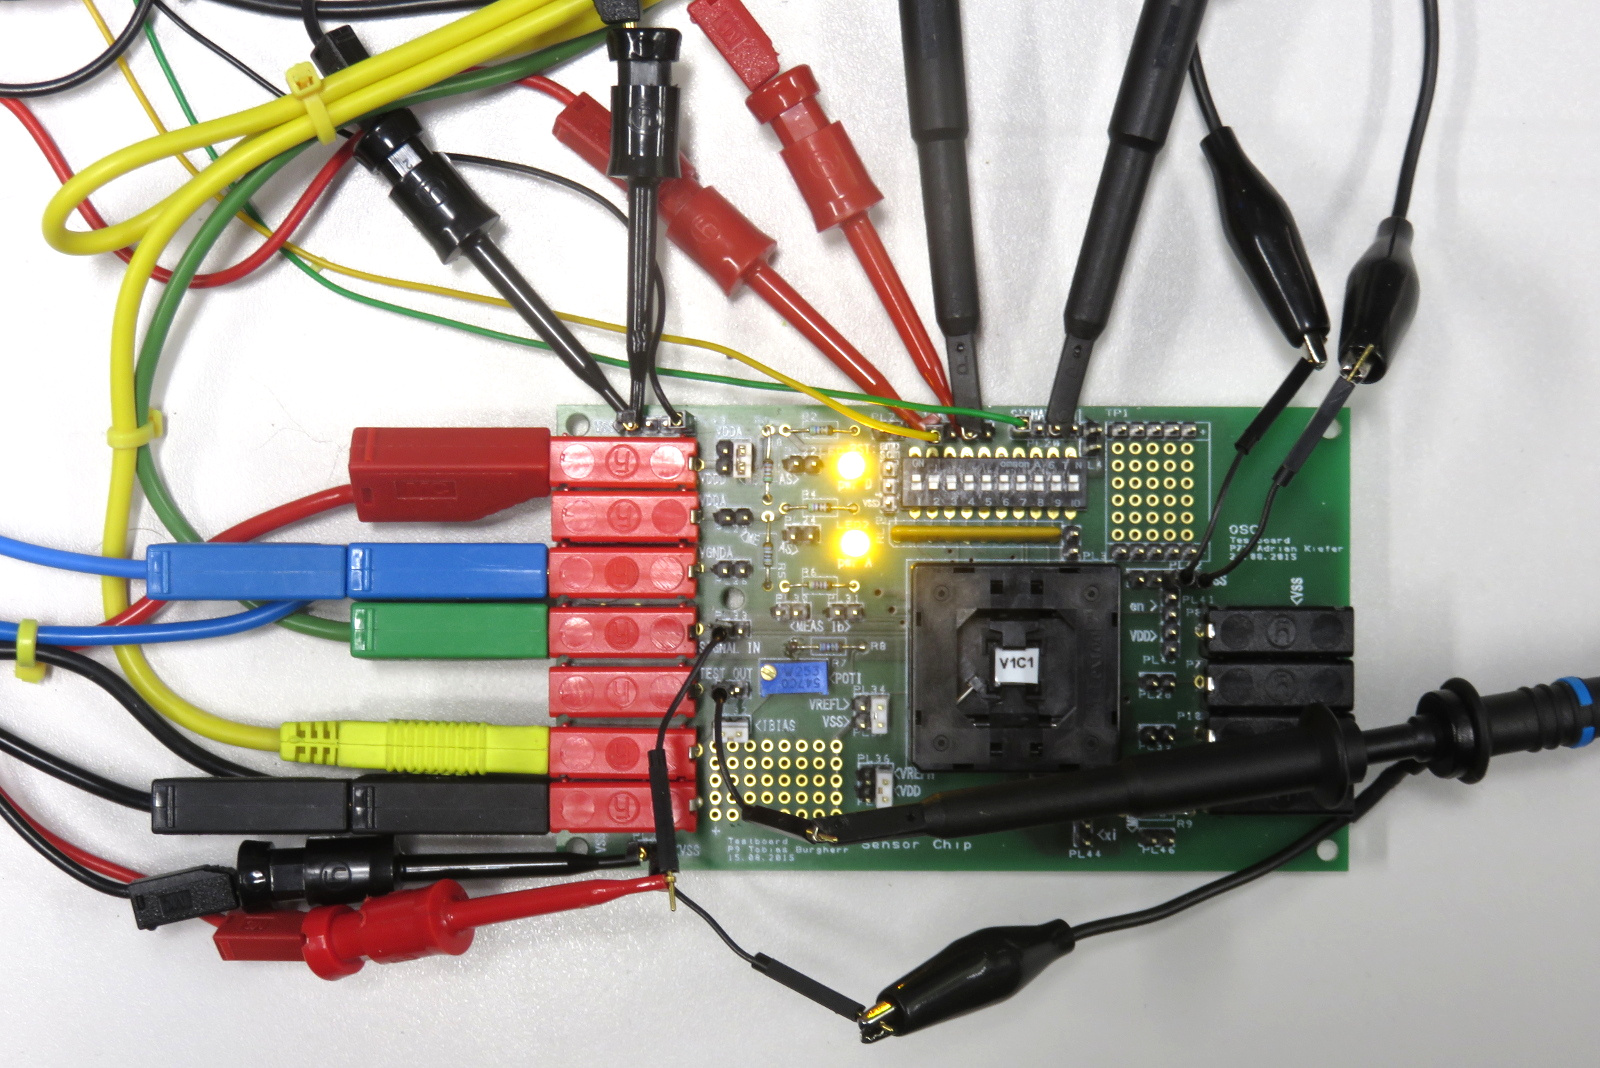
\includegraphics[width=\textwidth]{images/expSetup/testBoardConnected.jpeg}
    \caption{%
        The test board with all connections  as used in the configuration from
        figure \ref{fig:testBenchComplete}.%
    }
    \label{fig:testBenchConnected}
\end{figure}

\begin{table}
    \centering
    \caption{Sensor chip toplevel pins}
    \label{tab:topLevelPins}
    \scriptsize
    \sisetup{list-pair-separator = { or }}
    \rowcolors{2}{solarized-base3}{white}
    \begin{tabular}{>{\fontfamily{jkptt}\selectfont}l>{\fontfamily{jkptt}\selectfont}lp{30mm}lp{30mm}} \\
    %\begin{tabular}{>{\fontfamily{lmtt}\selectfont}l>{\fontfamily{lmtt}\selectfont}lp{30mm}lp{30mm}} \\
        \toprule
        \textnormal{\textsc{Pin \#}} & \textnormal{\textsc{Name}}                  & \textsc{Description} & \textsc{Value} & \textsc{Note} \\
        \midrule
        39 & vin                     & analog input signal                         & \SIrange{0.5}{2.5}{\volt} & \\
        25 & bit\_stream             & digital output signal                       & \SIlist{0;3}{\volt}       & \\
        34 & clk                     & clock                                       & \SIlist{0;3}{\volt}       & \\
        36 & sdm\_rst                & pulse to reset the $\Sigma\Delta M$         & \SIlist{0;3}{\volt}       & short pulse is enough (min $T_C$) \\
        41 & vgnda                   & analog ground                               & \SI{1.5}{\volt}           & \\
        48 & vrefh                   & high reference voltage                      & \SI{3}{\volt}             & \\
        47 & vrefl                   & low reference voltage                       & \SI{0}{\volt}             & \\
        46 & ibias                   & bias current                                & \SI{120}{\micro\ampere}   & $24 \cdot 5 \cdot 1$, internally reduced by 120 \\
        43 & sc\_amp\_vout\_test\_en & enables test output after preamp            & \SIlist{0;3}{\volt}       & \SI{0}{\volt}: off, \SI{3}{\volt}: on\\
        44 & sc\_amp\_vout\_test     & test output after preamp                    & \SIrange{0.5}{2.5}{\volt} \\
        33 & sc\_amp\_rst\_ext\_en   & enables external reset input for the preamp & \SIlist{0;3}{\volt}       & \SI{0}{\volt}: off, \SI{3}{\volt}: on\\
        32 & sc\_amp\_rst\_ext       & external reset input for the preamp         & \SIlist{0;3}{\volt}       & Internally synced to \signal{clk}. Needs \signal{en} signal. \\
        35 & sc\_amp\_pos\_neg\_amp  & positive or negative gain                   & \SIlist{0;3}{\volt}       & \SI{0}{\volt}: positive, \SI{3}{\volt}: negative \\
        28 - 31 & sc\_amp\_csel<3:0> & set gain                                    & \SIlist{0;3}{\volt}       & See table TODO \\
        27 & sc\_amp\_en             & enable preamp                               & \SIlist{0;3}{\volt}       & \SI{0}{\volt}: off, \SI{3}{\volt}: on\\
        26 & sah\_sdm\_en            & enable $\Sigma\Delta M$ S/H bock            & \SIlist{0;3}{\volt}       & \SI{0}{\volt}: off, \SI{3}{\volt}: on\\
        42 & vdda                    & analog positive power supply                & \SI{3}{\volt}             & \\
        37 & vddd                    & digital positive power supply               & \SI{3}{\volt}             & \\
        40 & vss                     & analog and digital negative power supply    & \SI{0}{\volt}             & \\
        \bottomrule
    \end{tabular}
    \sisetup{list-pair-separator = { and }}
\end{table}


% ---------------------------------------------------------------------------- %
\clearpage
\section{DC Power Supply}
\label{sec:dcPower}
% ---------------------------------------------------------------------------- %


The  \dcsupp~ has  three  independent direct  voltage  outputs. They are  used
to  supply \signal{VDDD},  \signal{VDDA},  \signal{VREFH}, \signal{VGNDA}  and
\signal{IBIAS}\footnotemark. Since the output current can only be limited, but
not  directly  set, the  bias  current  output  is  fed directly  through  one
of  the Keysight  tabletop  multimeters. The bias  current  is then  monitored
and  the  \dcsupp's  output  voltage  (and/or the  variable  resistor  on  the
test  board)  adjusted as  needed  to  achieve  the  desired bias  current  of
\SI{120}{\uA} as per Table \ref{tab:topLevelPins}.

\footnotetext{%
    All  \SI{3}{V} signals  are  fed from  the same  output  and bridged  with
    jumpers  on the  test board. This  concerns \signal{VDDD},  \signal{VDDA},
    \signal{VREFH} and \signal{VGNDA}.%
}


% ---------------------------------------------------------------------------- %
\section{Waveform Generators}
\label{sec:33120A}
% ---------------------------------------------------------------------------- %

The  \funcgen  s  are  controlled  remotely via  their  RS232  interface  from
a   computer  (through   RS232  $\rightarrow$   USB-A  adapters,   see  Figure
\ref{fig:rs232-usb})  and  a  Python script  (\code{33120A.py},  see  Appendix
\ref{app:chap:scripts} on page \pageref{app:chap:scripts}).

Before  usage, the  script needs  to be  configured. After connecting  via the
adapters,  the  two  waveform  generators  will  show  up  in  the  computer's
device  tree and  their identities  must  be entered  into the  script in  the
\code{SETTINGS} section:

\begin{figure}
    \centering
    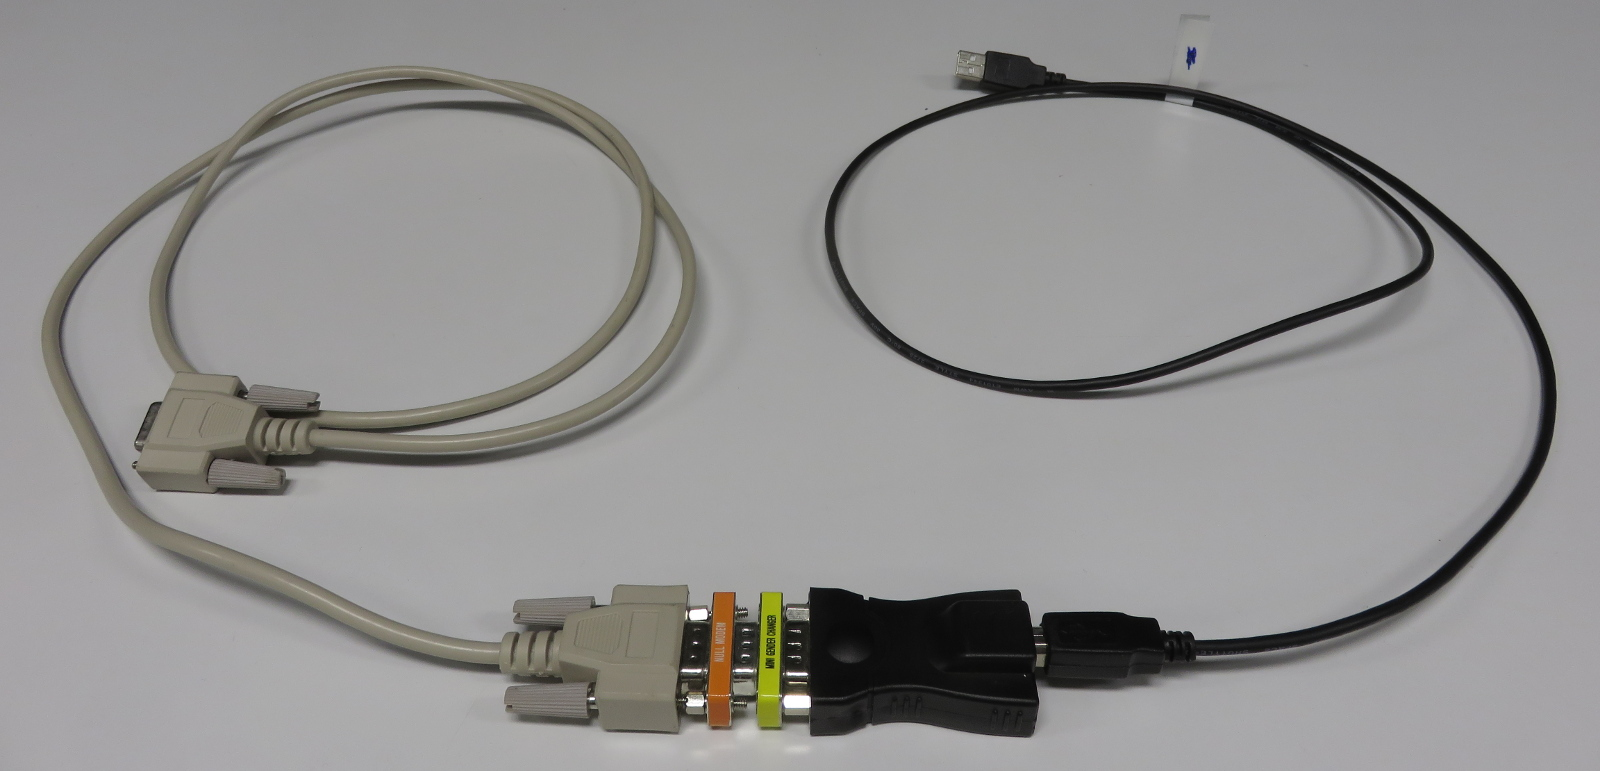
\includegraphics[width=0.5\textwidth]{images/expSetup/rs232-usb.jpeg}
    \caption{%
        One of  the two RS-232 to  USB adapters with cables. In  order for the
        adapter to properly  connect with the cables, both a  null modem and a
        gender changer are also used.%
    }
    \label{fig:rs232-usb}
\end{figure}

\begin{minted}{python}
# ------------------------------------------------------------------------ #
# SETTINGS                                                                 #
# ------------------------------------------------------------------------ #
CLK_DEVICE = '/dev/ttyUSB1'
DC_DEVICE  = '/dev/ttyUSB0'
\end{minted}

Whichever  device   registered  with  the   PC  first  will  have   the  lower
\code{ttyUSB<N>} number. If other  USB devices are connected  to the computer,
the numbers will of course be higher than \code{0} and \code{1}, respectively.

After successful configuration, the waveform generators can be controlled from
the command line like so\footnotemark:

\begin{minted}{shell}
$ ./33120A.py --clock=32e3
$ ./33120A.py --voltage=1.8
\end{minted}

The script will then select either the \signal{CLK} \signal{SIGNAL\_IN} device
and adjust  its output as specified. In  this case, the sampling  rate for the
test board  is set  to \SI{32}{\kilo\hertz}  and the DC  voltage on  the other
generator  is set  to \SI{1.8}{\volt}. More  information can  be found  in the
script itself.

The \signal{CLK} device  will always output a square wave  with voltage levels
\SI{0}{\volt} and \SI{3}{\volt}, as per table \ref{tab:topLevelPins}.

If needed,  the script can  easily be extended  to output any  other arbitrary
signal. The full  list of available commands  can be obtained from  the 33120A
operator's manual, which can be downloaded at \cite{ref:33120A:userGuide}.

\footnotetext{%
    This requires  the executable bit  to be set  on the file:  \code{chmod +x
    33120A.py}.%
}


% ---------------------------------------------------------------------------- %
\section{Multimeters}
\label{sec:34465A}
% ---------------------------------------------------------------------------- %

Three \emph{Keysight 34465A} multimeters are used. One for monitoring the bias
current, a second for monitoring the voltage for the input signal, and a third
one for monitoring the reference voltage (analog ground).

No  further  special  configuration  is  needed  on  the  multimeters  besides
setting  them  to   the  correct  measurement  modes   (voltage  and  current,
respectively). However, care must be taken when setting the range for the bias
current measurement. \SI{120}{\micro\ampere} is right  on the edge between two
measurement ranges (\si{\micro\ampere}  and \si{\milli\ampere}, respectively),
and  the measurement  results between  these two  ranges are  not identical. A
difference  of  about  \SI{7}{\micro\ampere}  was typically  observed  in  our
experiments. In our measurements, the device is set to the millivolt range.

The    user   manual    for   the    multimeter   can    be   downloaded    at
\cite{ref:34460:userGuide}.


% ---------------------------------------------------------------------------- %
\section{Oscilloscope}
\label{sec:oscilloscope}
% ---------------------------------------------------------------------------- %

The oscilloscope  is used for  monitoring the clock,  the bit stream,  and for
acquiring measurment data for the preamp via the test output pin.

% ---------------------------------------------------------------------------- %
\subsection{Clock and Bit Stream}
\label{subsec:clockBitstream}
% ---------------------------------------------------------------------------- %

Monitoring  the clock  and  bit stream  is straightforward: The  oscilloscopes
probes are connected  to the corresponding pins on the  test board as depicted
in Figure \ref{fig:clockBitStreamProbes}.

\begin{figure}
    \centering
    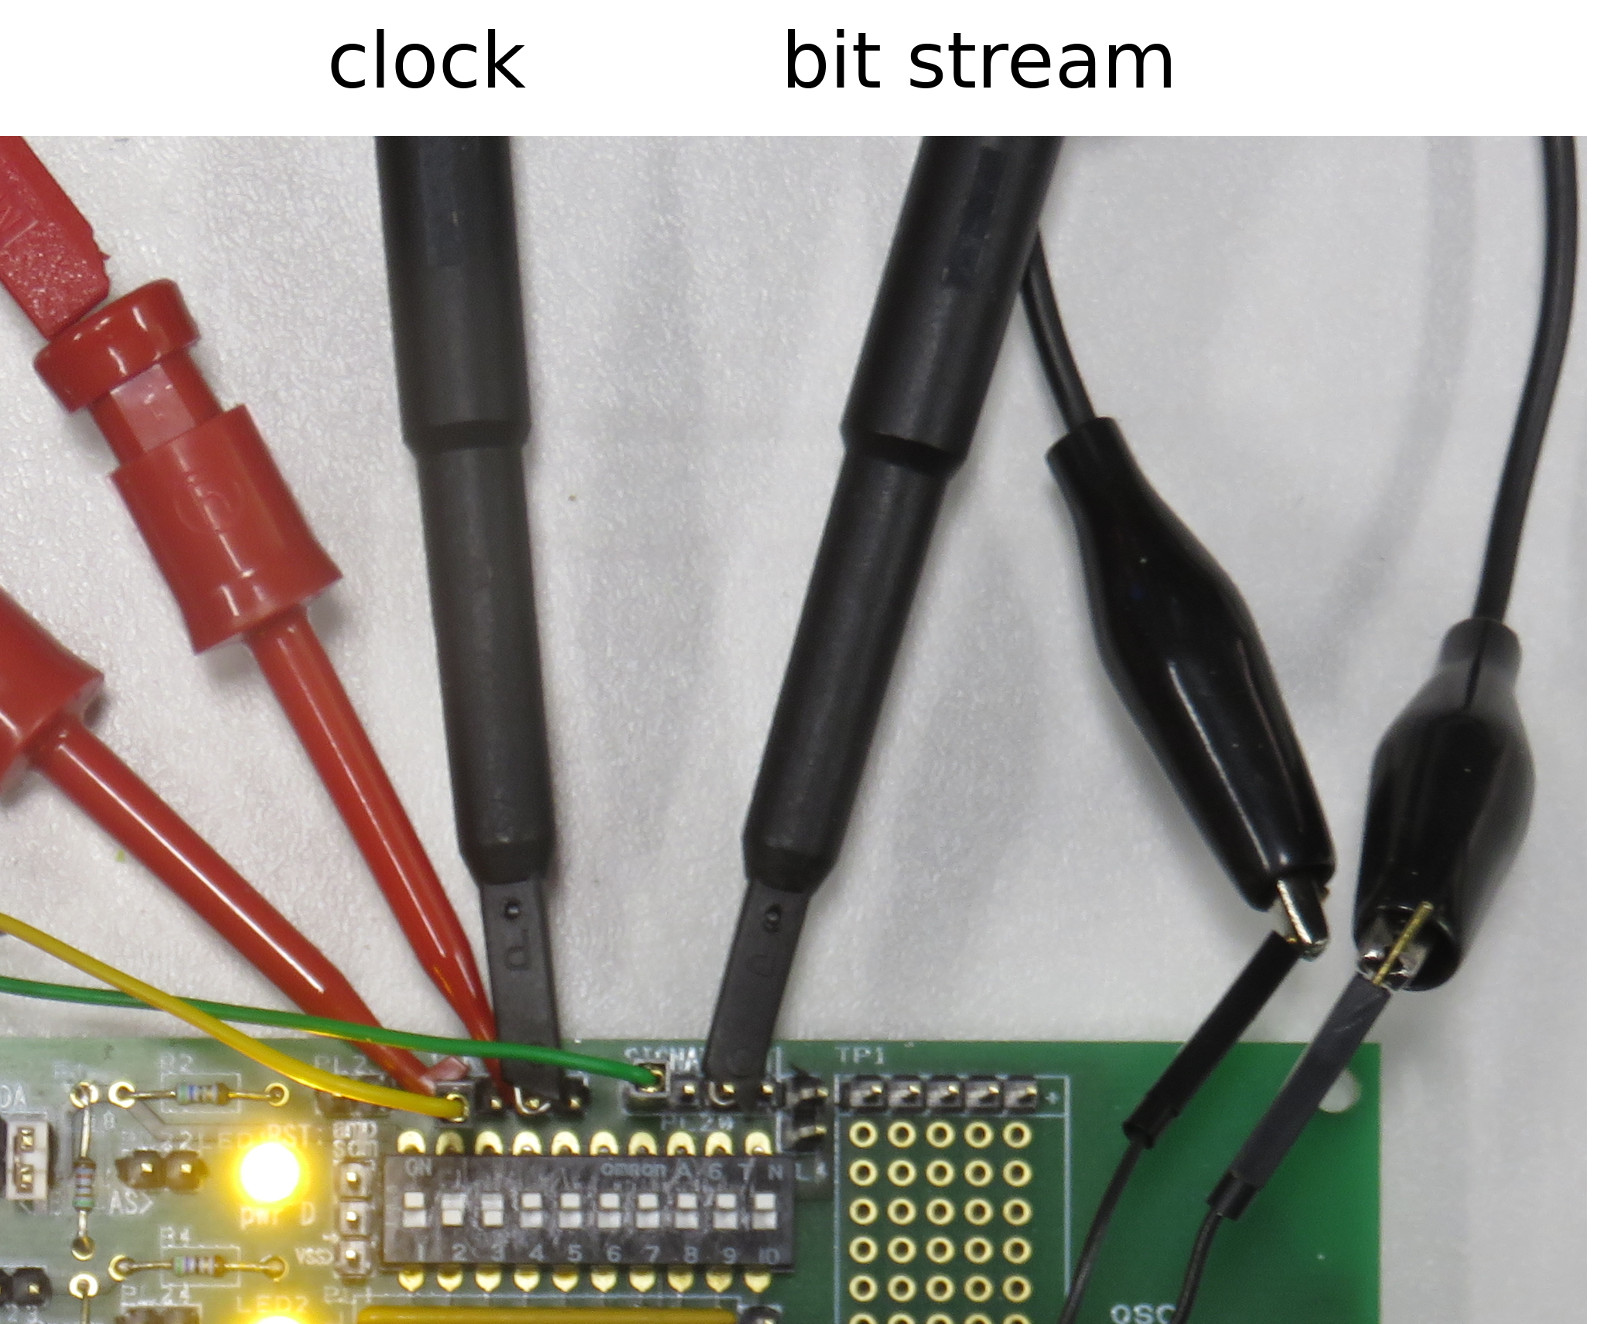
\includegraphics[width=0.67\textwidth]{images/expSetup/testBoardOsciBitStreamClkProbes.jpeg}
    \caption{%
        Clock and  bit stream  monitoring. \emph{Note}: Since the  clock input
        pins are not interconnected, and both the \raspi~ and the oscilloscope
        are connected  to one clock pin  each, two supply clamps  (in red) are
        used on the clock input via a Y splitter from the coaxial cable coming
        from the signal  generator. This is not strictly  necessary, but makes
        connecting the  probes, plugs  and supply  clamps easier  without them
        slipping off the pins.%
    }
    \label{fig:clockBitStreamProbes}
\end{figure}


If the clock  and bit stream do not  look as they should, common  errors are a
disabled sample-and-hold circuit, an incorrect clock voltage (particularly its
DC offset) or an incorrect bias current.


% ---------------------------------------------------------------------------- %
\subsection{Analog Measurements of Preamp}
\label{subsec:analogMeasurements}
% ---------------------------------------------------------------------------- %

Performing  analog measurements  of  the pre-amplifier  is  a noticeably  more
involved process. A measurement  probe is connected to the test  output pin on
the test board as shown in Figure \ref{fig:testOutProbe}.

\begin{figure}
    \centering
    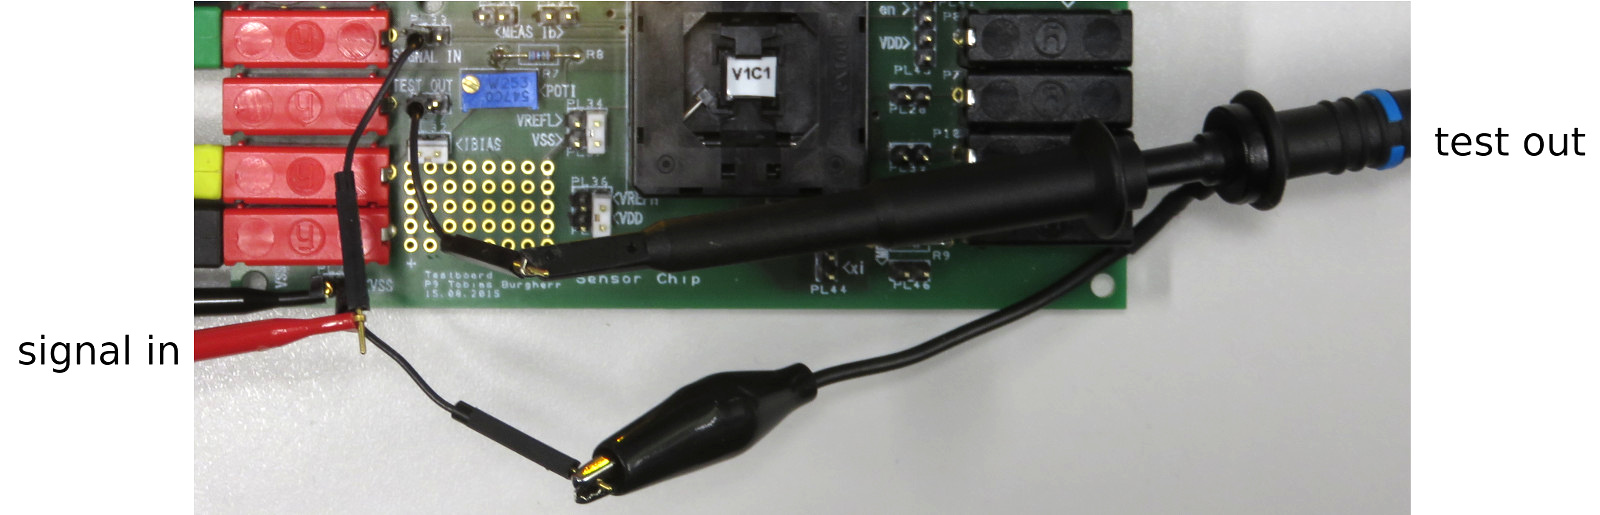
\includegraphics[width=\textwidth]{images/expSetup/testBoardOsciTestOutProbe.jpeg}
    \caption{%
        Measuring preamp  output. On the left,  the tip  of the clamp  for the
        input signal can be seen, coming from one of the waveform generators.%
    }
    \label{fig:testOutProbe}
\end{figure}


Besides the  oscilloscope itself,  a laptop  is used  to remotely  control the
oscilloscope and  the two function generators  (one for the clock  and for the
input signal, respectively).

The  connection  between  the  oscilloscope  and  the  laptop  is  established
via  ethernet,  with  each  device  being assigned  a  fixed  IP  address. The
laptop  is configured  to match  the oscilloscope's  network settings. How  to
configure the laptop is outlined in Section \ref{sec:laptop}, starting on page
\pageref{sec:laptop}.


After  having  successfully  established   a  connection  between  laptop  and
oscilloscope, a  collection of  three scripts  is used  to configure  the test
setup and acquire the measurement data:

\begin{itemize}\tightlist
    \item 
        A shell wrapper script, 
    \item
        \code{33120A.py}: For controlling the waveform generators (see section
        \ref{sec:33120A})
    \item 
        \code{initWaveRunner.py}: resets and initializes the oscilloscope with
        a given configuration.
    \item 
        \code{configWaveRunner.py}:   configures  various   settings  on   the
        oscilloscope.
    \item 
        \code{acquireWaveRunnerData.py}:   performs   measurements   via   the
        oscilloscope.
\end{itemize}


The  python  scripts   are  mostly  self-explanatory  with   aid  of  LeCroy's
documentation   found  in   \cite{ref:WR:opMan},  \cite{ref:WR:gettingStarted}
and    \cite{ref:WR:remoteControl}. A   detailled    explanation   of    their
implementation   will   therefore   be   ommitted,   and   instead   a   brief
outline   of   each   script's   purpose  and   usage   is   provided.    They
can    be    found    in    Appendices    \ref{sec:app:waveRunner:initialize},
\ref{sec:app:waveRunner:config} and \ref{sec:app:waveRunner:acquire}, starting
on page \pageref{sec:app:waveRunner:initialize}.

The initialization script  resets the oscilloscope and  configures the trigger
channel, trigger level, trigger flank,  time division, which traces to display
and sets the DC coupling of the channels to a resistance of \SI{1}{\mega\ohm}.

\code{configWaveRunner.py} is used  to set the horizontal  (time) and vertical
(voltage) divisions on the oscilloscope,  as well as the vertical offset. This
is necessary because the oscilloscope will only store measurement data for the
section of any given trace which is being shown on the display. Any meaurement
points which  are not on  the oscilloscope's display will  not be stored  in a
measurement file. Although this is a  bit cumbersome and counter-intuitive, it
does have  the advantage that  one can see  immediately if something  has been
incorrectly configured during  the measurement process, as  the display output
will then be incorrect.

\code{acquireWaveRunnerData.py}  executes   the  actual  measurement   on  the
oscilloscope  for a  given channel. The  measurement results  are stored  in a
text file, which is then downloaded to the laptop.

The entire process is controlled via  a shell wrapper script. This script will
be explained  in more  detail in the  following paragraphs. There  are various
versions of  the script for  different measurements,  but they all  follow the
same outline.

For each measurement run, the chip  number, the gain (sign and absolute value)
and the channel which  is connected to the test output on  the test board must
be set.  Furthermore, the target directory  in which the measurement data will
be  stored on  the PC  is configured  according to  the chip  number and  gain
settings.   There is  also an  optional  flag for  resetting the  oscilloscope
before performing the measurements, if so desired. In the following example, a
gain of \code{+1} will be measured for chip number 1:

\begin{minted}{shell}
CHIP='chip01'
SIGN='+'
CHANNEL='3'
GAIN='1'
DATA_DIR="data/${CHIP}Gain${SIGN}$(printf '%02d' $GAIN)"
RESET='0' # 1: reset and initialize the oscilloscope
\end{minted}

Before actually performing any measurements,  the script will display a series
of  messages to  the user,  accounting  for a  few quirks  of the  setup. This
minimizes  user  error  and  ensures  that time  is  not  wasted  on  unusable
measurements due to erroneous configurations.

The first message concerns the number  of sample points which the oscilloscope
is set to acquire. This  must be set to \num{500} kilo  samples per second, as
shown in  Figure \ref{fig:kilosamples}. If this  is not done,  the measurement
data will exhibit strong quantization errors, resulting in unusable data.

The  next  two  messages  concern  the  measurement  files  which  are  stored
on   the  oscilloscope.    They   follow   a  naming   scheme   of  the   form
\code{C<ChannelNo>Trace<FileNo>.txt},   starting   at  file   zero   (example:
\code{C2Trace00002.txt}  for the  third  file for  channel 2). Each  channel's
counter is independent of the  other channels' counters. The counter for these
file names  will keep incrementing,  regardless of any remote  commands, until
they are manually reset via the Oscilloscope's graphical user interface.

To avoid needing to manually reset  this counter between each measurement, the
script maintains  its own  counter to  match the  oscilloscope's. Between each
measurement  run (i.e.  each script  execution), manual  intervention via  the
oscilloscope's GUI is necessary to reset the oscrilloscope's counter, as shown
in figure \ref{fig:fileCounterReset}.

\begin{figure}
    \centering
    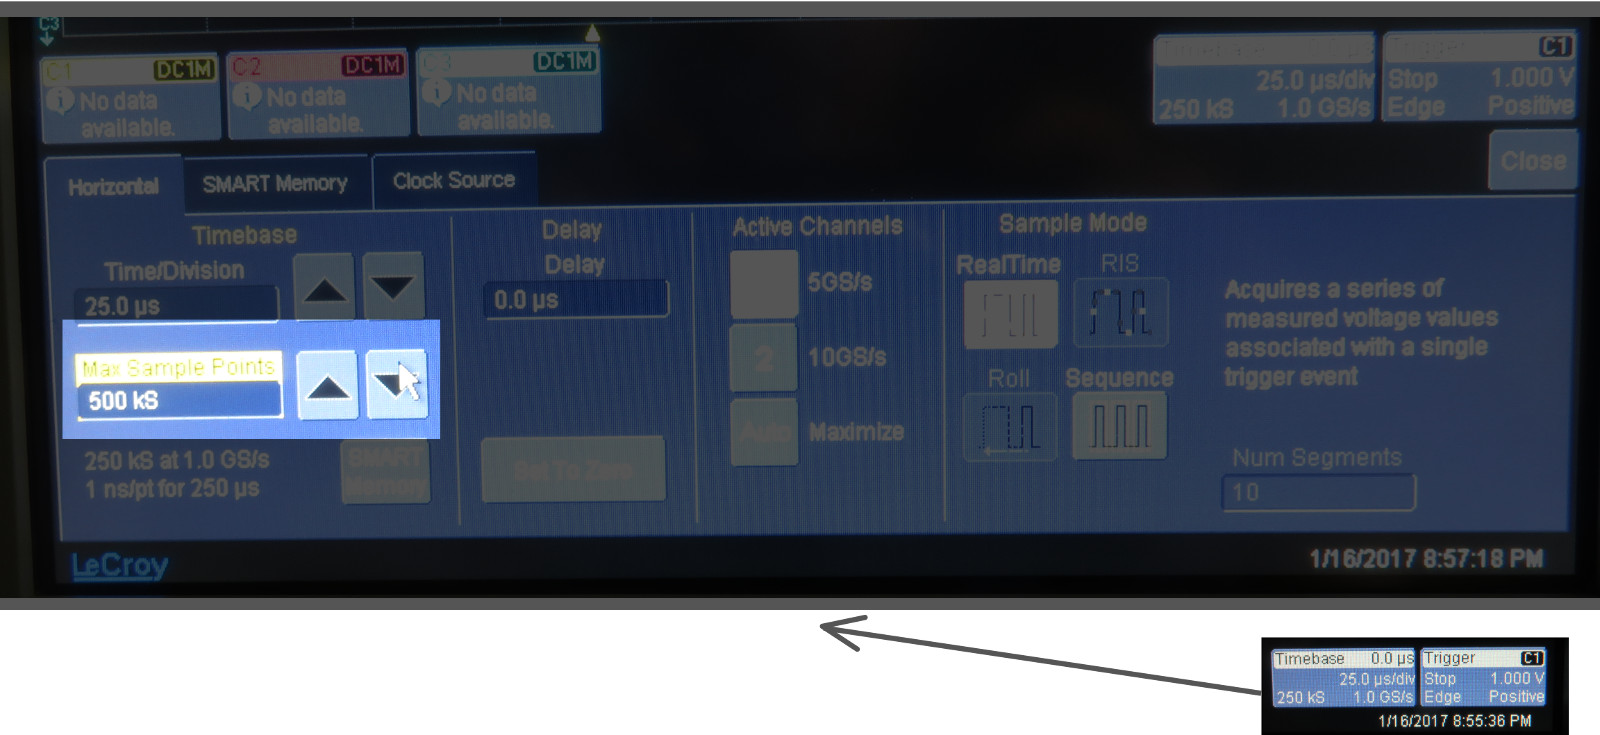
\includegraphics[width=\textwidth]{images/expSetup/setSamples.jpeg}
    \caption{%
        Set sample rate on oscilloscope. Click the \emph{Timebase} icon on the
        bottom right of  the screen, then adjust the  \emph{Max Sample Points}
        setting (highlighted)  to \num{500} kilo  samples in the  dialog which
        opens.%
    }
    \label{fig:kilosamples}
\end{figure}


\begin{figure}
    \centering
    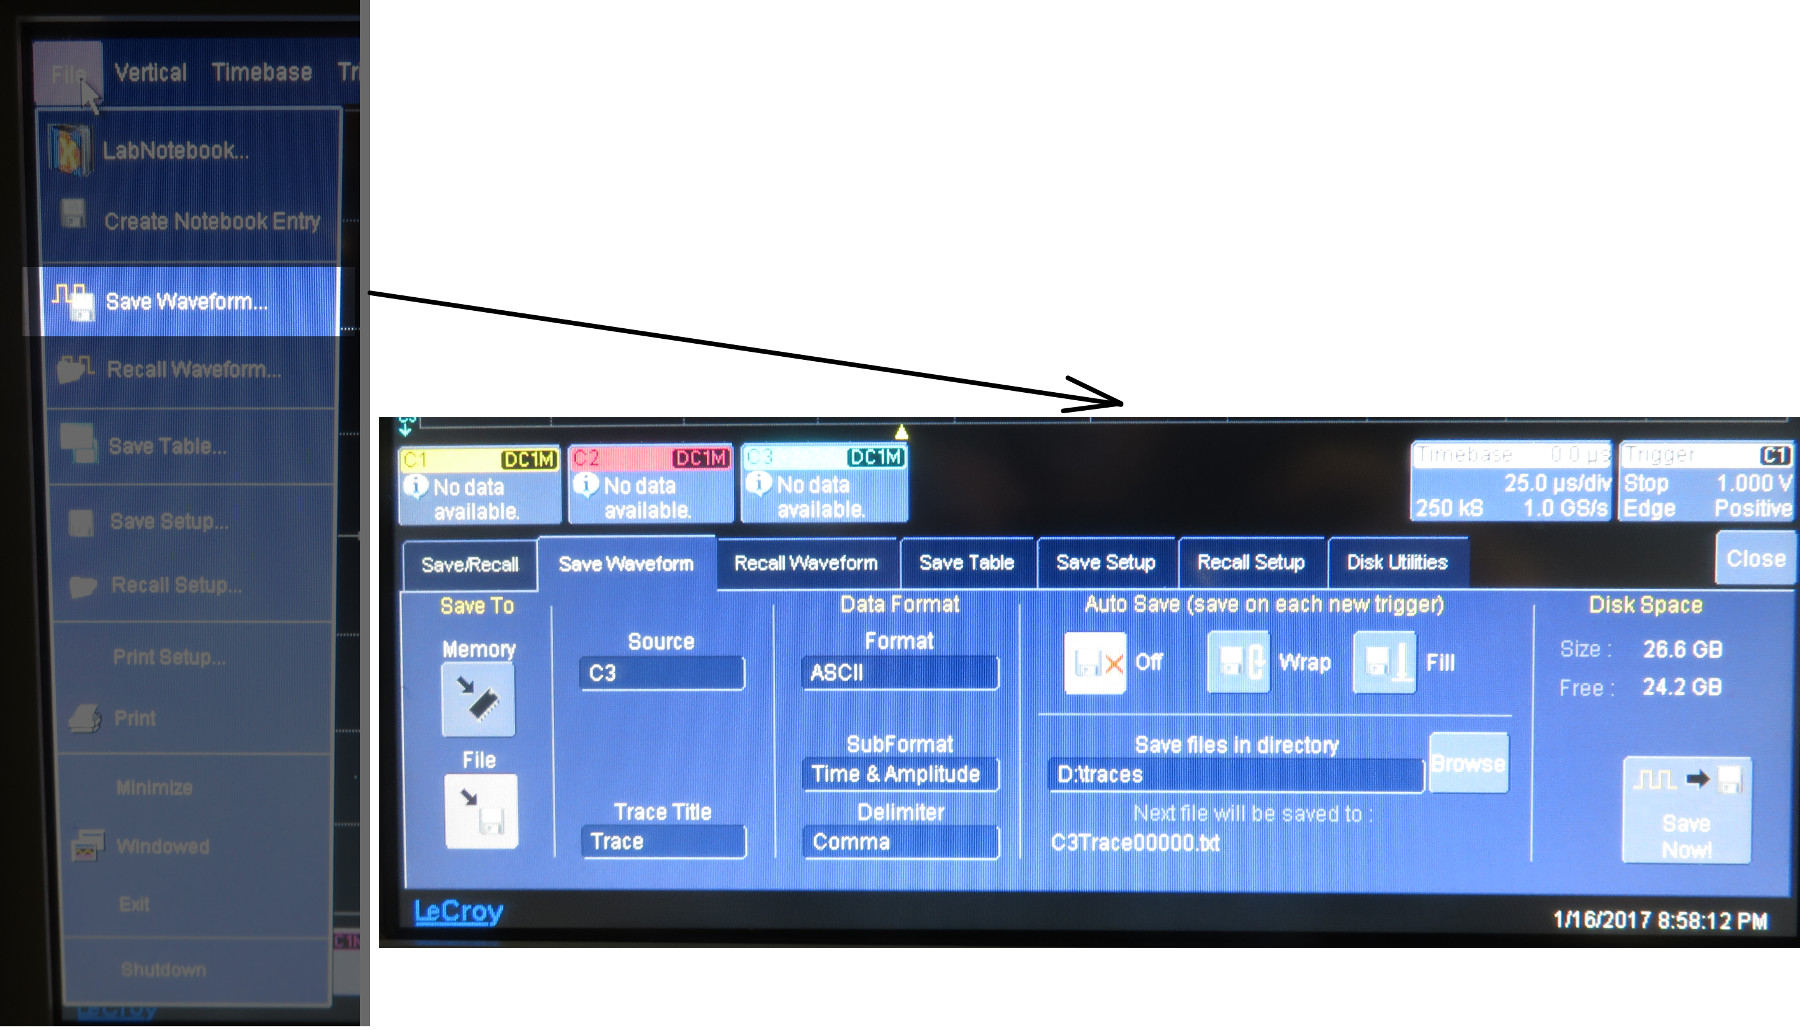
\includegraphics[width=\textwidth]{images/expSetup/resetFilename.jpeg}
    \caption{%
        Resetting the file counter  on the oscilloscope. Click the \emph{File}
        menu at  the top of the  screen, then select the  \emph{Save Waveform}
        dialog.  If  the oscilloscope has  been reset, select  the appropriate
        channel, DataFormat (ASCII)  and the directory where the  files are to
        be saved (which must correspond with the directory set in the wrapping
        shell script). After initial configuration, this dialog must be opened
        between each script run to reset the file name counter, but no further
        intervention is necessary.%
    }
    \label{fig:fileCounterReset}
\end{figure}

The  next   step  in   the  script's  execution   is  performing   the  actual
measurements. Various  settings  are  hard-coded  into  the  script  for  this
purpose. Firstly,  the   appropriate  time   divisions  for   configuring  the
oscilloscope's display\footnotemark:

\begin{minted}{shell}
declare -A timeDivs
timeDivs[32e3]='5'
timeDivs[96e3]='2.5'
timeDivs[256e3]='1'
\end{minted}

\footnotetext{
    These  values were  obtained by  trial and  error to  generate a  sensible
    display output.
}

Additionally, the list of amplitudes to be used for the input voltages:

\begin{minted}{shell}
declare -a ampls=(0.5 0.7 0.9 1.1 1.3 1.5 1.7 1.9 2.1 2.3 2.5)
\end{minted}

Each input voltage (including the gain's  sign) is assigned a voltage division
and a time division for the oscilloscope's display settings\footnotemark:

\begin{minted}{shell}
declare -A voltDivs
voltDivs[+0.5]='200'
voltDivs[+0.7]='200'
voltDivs[+0.9]='100'
...
voltDivs[-2.1]='100'
voltDivs[-2.3]='200'
voltDivs[-2.5]='200'

declare -A offsets
offsets[+0.5]='-1000'
offsets[+0.7]='-1100'
offsets[+0.9]='-1200'
...
offsets[-2.1]='-1200'
offsets[-2.3]='-1100'
offsets[-2.5]='-1000'
\end{minted}

\footnotetext{
    Also determined by trial and error.
}

Now, everything is  ready to perform the measurements, tying  together all the
scripts and configurations which have been mentioned so far:

\begin{minted}{shell}
i=0
mkdir -p "$DATA_DIR"
for clk in 32e3 96e3 256e3;do
    ./33120A.py --clock=$clk
    sleep 0.25 # give the function generator time to settle
    ./configWaveRunner.py --tdiv=${timeDivs[$clk]}

    # Run through DC ramp
    for ampl in "${ampls[@]}";do
        ./33120A.py --voltage="$ampl"
        sleep 0.25
        ./configWaveRunner.py \
            --vdiv=${voltDivs[${SIGN}${ampl}]} \
            --offset=${offsets[${SIGN}${ampl}]}
        sleep 2 # Give the oscilloscope time to do configure
        printf 'Acquiring trace for %s Hz and %s V\n' $clk $ampl
        ./acquireWaveRunnerData.py \
            --channel="C${CHANNEL}" \
            --remotefile="C${CHANNEL}Trace$(printf '%05d' $i).txt" \
            --localfile="${DATA_DIR}/${CHIP}-gain${SIGN} \
                $(printf '%02d' ${GAIN})-${fsStrings[$clk]}-${ampl}V.txt"
        i=$((i+1))
    done
done
\end{minted}

For each  measurement series, one  target directory  is created, in  which one
file for each clock frequency and  input voltage is generated. These files can
then be processed as outlined in Chapter \ref{chap:results}.


% ---------------------------------------------------------------------------- %
\section{Raspberry Pi}
\label{sec:raspi}
% ---------------------------------------------------------------------------- %

Installation of the operating system  is fairly straight forward. We recommend
using the NOOBS \cite{ref:raspinoobs} OS installer.

The first thing to  do is to set up SSHD so that  a remote connection with the
\raspi  can be  established.  This  isn't strictly  required, if  preferred, a
monitor and keyboard  connected directly to the \raspi~ can  also be used. The
scripts  used  measuring measuring  data  and  transferring  the data  to  our
computers do rely on SSH, though.

cmake and gcc  need to be installed, if they're  not already. To check whether
the programs exist, type the following into a terminal:

\begin{minted}{shell}
$ cmake --version
$ gcc --version
\end{minted}

If either return a ``command not found''  then  you  will need to install them
with:
\begin{minted}{shell}
$ sudo apt-get install cmake
$ sudo apt-get install gcc
\end{minted}

The \raspi~ has dhcpcd running by  default, which means it  will automatically
lease an IP as  soon as it is connected to the  network. The \raspi~ will need
to be  whitelisted by the  IT department  in order to  be able to  establish a
remote connection.   This involves  finding out its  MAC address. This  can be
done with the following command:

\begin{minted}{shell}
$ sudo ifconfig
eth0      Link encap:Ethernet  HWaddr b8:27:eb:e2:d2:c6  
          inet addr:10.84.130.16  Bcast:10.84.130.255  Mask:255.255.255.0
\end{minted}

\code{HWaddr b8:27:eb:e2:d2:c6} is the information needed.

The software for recording the bit stream  can be found in the svn repository.
It can be copied to the \raspi~ using SSH:

\begin{minted}{shell}
$ scp -r path/to/software pi@10.84.130.16:/home/pi
\end{minted}

This will  place the software folder into the home folder on the \raspi. Next,
open a  terminal  and navigate into the software folder. Execute the following
commands to configure and compile the software:
\begin{minted}{shell}
$ mkdir build
$ cd build
$ cmake -DCMAKE_BUILD_TYPE=Release ../
$ make
\end{minted}

This  will  produce an  executable  \textit{bitstream}.   You can  initiate  a
measurement by executing:

\begin{minted}{shell}
$ sudo ./bitstream
\end{minted}

If the chip is  connected  and running properly, the program will exit after a
few seconds and  a new file \textit{bit\_stream.txt} will exist in the folder.

On the hardware side, not much configuration is needed. A dedicated cable with
a 40-pin plug has been created to easily connect the \raspi~ with the required
pins on the test board (bit stream,  clock and ground). This cable is shown in
Figure \ref{fig:raspiCable}, connected to the test board.

\begin{figure}
    \centering
    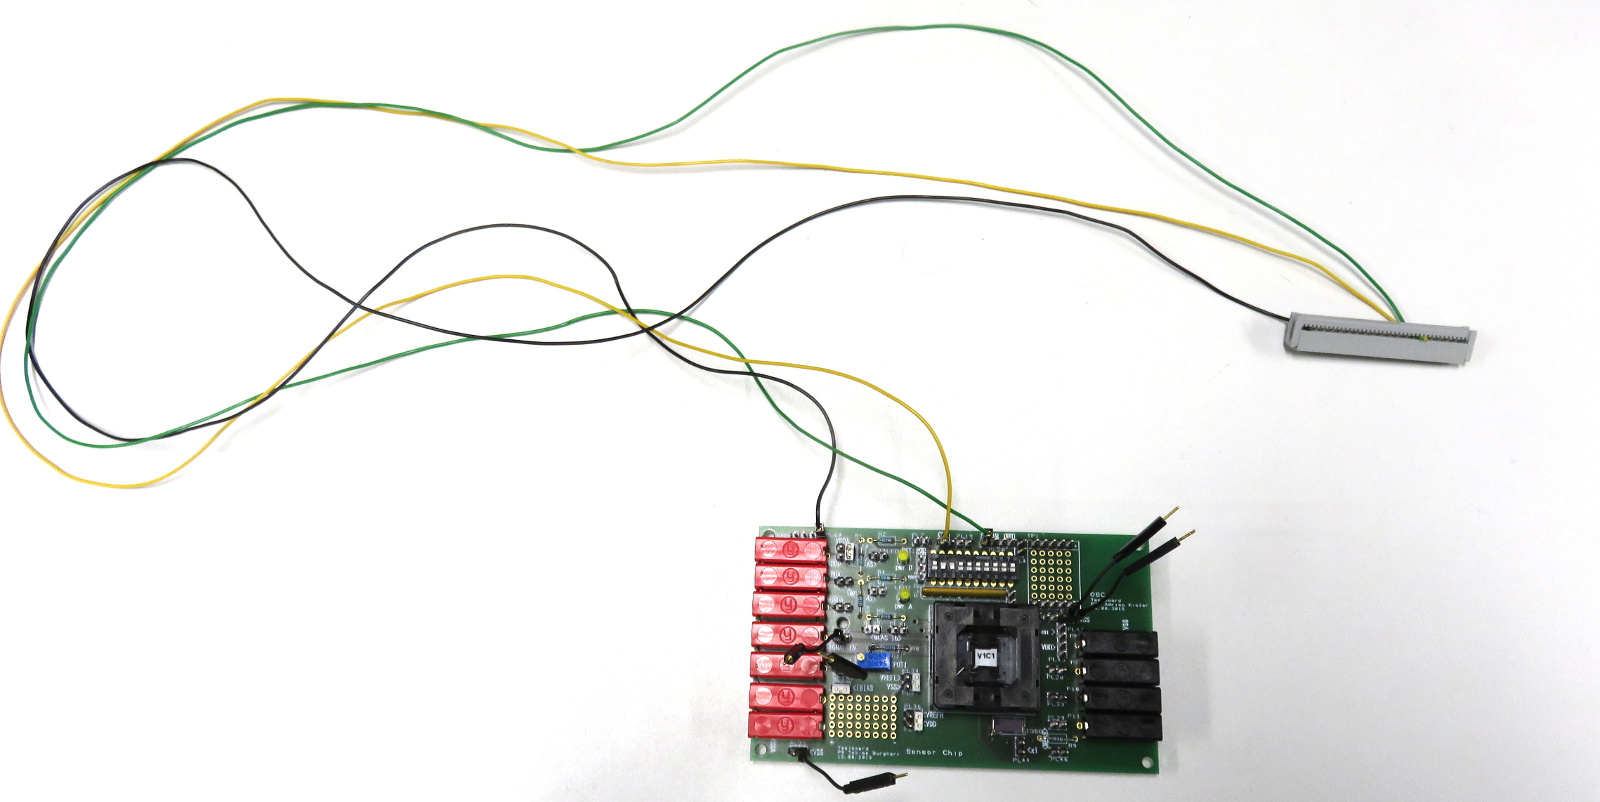
\includegraphics[width=0.75\textwidth]{images/expSetup/raspiCable.jpeg}
    \caption{%
        \raspi~ cable with  wires for clock, ground and  bit stream, connected
        to the test board%
    }
    \label{fig:raspiCable}
\end{figure}


% ---------------------------------------------------------------------------- %
\section{Laptop}
\label{sec:laptop}
% ---------------------------------------------------------------------------- %

This section outlines the prerequisites, configuration and usage of a computer
which is  used to  control the  measurement process. A laptop  is used  in our
case, but  any computer with  a network  and at least  two USB ports  (for the
waveform generators) can be used.


% ---------------------------------------------------------------------------- %
\subsection{Prerequisites}
\label{subsec:laptop:prereqs}
% ---------------------------------------------------------------------------- %

For controlling the test bench, a laptop running Linux is used. Fundamentally,
other configurations are  likely also possible, but have  not been tested. Any
Bash  version 4.0  and newer  should be  able to  execute the  wrapper scripts
(associated arrays must be supported). Even Windows  10 has Bash as well these
days \cite{ref:W10:bash}, for the adventure-minded.

Besides Bash  $\geq4.0$ support, Python  3 must  be installed, along  with the
following modules:

\begin{itemize}\tightlist
    \item
        \code{serial}: For communicating with the waveform generators
    \item
        \code{vxi11}: For communicating with the oscilloscope
    \item
        \code{sigmadelta}: For processing the bit stream
\end{itemize}

These  modules can  either be  installed via  pip or  via your  distribution's
package manager.

The \raspi~  is remote-controlled via SSH  from the laptop. In order  to avoid
having to  type in  a password  for each SSH  connection attempt  (which would
become cumbersome very  quickly), SSH key files are used.   For information on
how to  generate and install  SSH keys, there  are many online  resources, for
example the Arch Linux Wiki \cite{ref:archWiki:SSH}.


% ---------------------------------------------------------------------------- %
\subsection{Ethernet Configuration}
\label{subsec:laptop:netconf}
% ---------------------------------------------------------------------------- %

For  communicating  with  the  oscilloscope via  ethernet,  a  static  network
connection is used,  corresponding to the settings on  the oscilloscope (which
can  be checked  via  the  network dialog  in  the  oscilloscope's Windows  XP
operating system).

On the  machine used in our  measurements (a Macbook Pro  running Arch Linux),
this is done via \code{netctl} as follows\footnotemark:

\begin{minted}{text}
Description='WaveRunner Oscilloscope Ethernet Connection'
Interface=ens9                                                                                                                                                                                            
Connection=ethernet                                                                                                                                                                                       
IP=static                                                                                                                                                                                                 
Address=('169.254.14.1/16')                                                                                                                                                                               
\end{minted}

\footnotetext{
    Make  sure   \emph{not}  to  set   a  \code{Gateway}  parameter   in  this
    configuration,  or the  laptop will  try to  access the  internet via  the
    oscilloscope, which will obviously fail.
}

The  \code{Interface} parameter  needs to  be  adjusted to  the machine  which
is  being  used. A  list  of   available  interfaces  can  be  displayed  with
\code{ip  addr}  on  systems  which have  the  \code{iproute2}  utility  suite
\cite{ref:iproute2}  installed,  or with  \code{ifconfig}  \cite{ref:ifconfig}
on  other  *nix  operating  systems. For  further  information,  consult  your
distribution's manpages.
